%% content.tex
%%
\chapter{Illustrationen}
\label{ch:illustrationen}

\section{Bilder}
\label{ch:illustrationen:sec:images}

Bilder kann man natürlich auch in Arbeiten integrieren.
Für Fotos und Ähnliches unterstützt PDF-\LaTeX{} direkt \verb|jpg| und \verb|png|, ansonsten empfiehlt es sich Vektorgrafiken zu verwenden und diese als \verb|pdf| zu speichern.
Sollte ein Bild einmal zu viel weißen Raum um sich haben, so kann man mit dem Werkzeug \verb|pdfcrop| das Bild automatisch ausschneiden\cite{pdfcrop}.

\begin{figure} [ht]
\centering
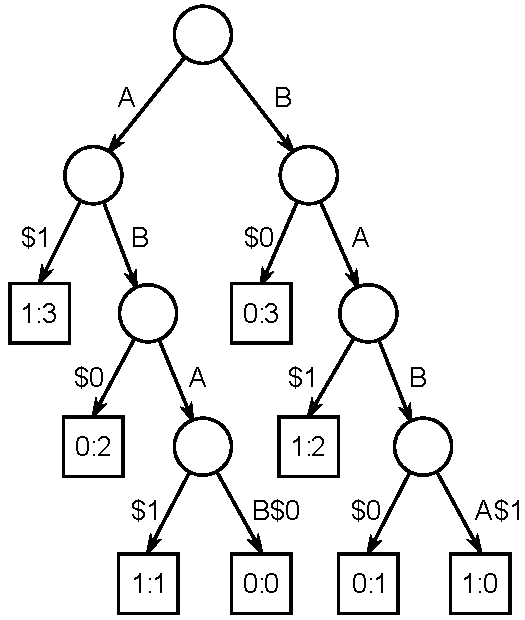
\includegraphics[width=.4\textwidth]{images/Suffix_tree_ABAB_BABA}
\caption{Beschreibung/Beschriftung des Bilds}
\label{fig:bild1}
\end{figure}

Mit Hilfe eines Labels kann man sich dann im Text auf diese Grafik (\ref{fig:bild1}) beziehen. 

\section{Tabellen}
\label{ch:illustrationen:sec:tables}

Seite \pageref{tab:beispieltabelle} enthält Beispieltabelle \ref{tab:beispieltabelle}.
In jedem \LaTeX{}-Buch finden sich gute Anleitungen zum Erstellen von Tabellen.
Komplexere Tabellen können in Excel vorgefertigt und mit Excel2LaTeX, einem Add-in von Excel, nach LaTeX konvertiert werden.

\begin{table}[h]
\begin{center}
\begin{tabular}{|l|l|l|}
	A & B & C \\\hline
	x & x & x \\
	x & x & x
\end{tabular}
\end{center}
\caption{Eine kleine Beispieltabelle}
\label{tab:beispieltabelle}
\end{table}

\section{Formeln}
\label{ch:illustrationen:sec:formula}

sec Formeln lassen sich in der Umgebung  \verb|math| erzeugen.
Die Kurz- Schreibweise lautet \verb|\( a^2+b^2=c^2 \)|;  hierbei steht die Formel dann im laufenden Text: \( a^2+b^2=c^2 \).
Die kürzeste Form ist mit zwei \verb|$| um die Formel, z.B.~so: Wasser ist H$_2$O.

Mit der Schreibweise \verb|\[ y=x^2 \]| wird die Formel mittig in einer eigenen Zeile gesetzt, z.B.

\[y = x^2 \]

Formeln in der Umgebung \verb|equation| werden mittig in einer eigenen Zeile gesetzt und fortlaufend nummeriert:

\begin{equation}
x_{1,2} = \frac{-b\pm\sqrt{b^2-4ac}}{2a}
\label{mitternachtsformel}
\end{equation}
Wenn wir z.B.~über die beliebte Mitternachtsformel (Gleichung \ref{mitternachtsformel}) Details im umliegenden Text schreiben wollen, lässt sich diese wie ein Bild referenzieren.

\section{Quellcode}
\label{ch:illustrationen:sec:code}

Quellcode und ähnlich zu formatierende Texte können mit \verb|verbatim| in einer Umgebung gesetzt werden.

\begin{verbatim}
Dieser Text ist in Schreibmaschinenschrift
\end{verbatim}

Schöner geht es mit dem \verb|listings|-Paket, das Quelltext auch entsprechend formatiert.
Dazu kann man in der Präambel die Sprache angeben, in der die Quellcodes geschrieben sind.

\begin{lstlisting}
public class Hello {
    public static void main(String[] args) {
        System.out.println("Hello World");
    }
}
\end{lstlisting}

Im Text gibt man Wörter am Besten als \verb|\verb##| an, dabei erwartet \LaTeX{} zweimal das gleiche Zeichen als Begrenzer.
Im Beispiel ist dies die Raute \verb|#|, man kann aber ein anderes Zeichen nehmen, z.B. das Plus .

\section{Text}
\label{ch:illustrationen:sec:text}

Text kann mit dem Befehl \verb|\emph{}| \emph{hervorgehoben} werden.
Falls in einem Satz ein Punkt vorkommt, macht man vor ihm kein Leerzeichen sondern eine Tilde (\verb|~|), denn dann fügt \LaTeX{} den korrekten Abstand ein, z.B.~so.

\begin{verbatim}
z.B.~so
\end{verbatim}

In der Präambel der vorliegenden tex-Datei gibt es den Befehl \verb|hypenation|, der zur Silbentrennung da ist.
\LaTeX{} verfügt zwar über  eine eingebaute Silbentrennung, die jedoch bei manchen Wörtern falsch trennt.
Damit diese Wörter korrekt getrennt werden, gibt man sie dann mit dem Befehl in der Präambel an\footnote{Das Wort \emph{Silbentrennung} ist hier das Beispiel}.

Fußnoten werden mit dem Befehl \verb|footnote| mitten in den fortlaufenden Text eingefügt. \footnote{Wie man schon im vorherigen Absatz sehen konnte.}.

In wissenschaftlichen Arbeiten muss man des öfteren andere Arbeiten zitieren.
Dazu nutzt man den Befehl \verb|\cite{name}|.
In eckigen Klammern kann man noch die Seitenzahl angeben, falls notwendig.
Der Name ist ein Schlüssel aus der Datei \verb|bibliography.bib| \cite[S.~10]{kopka}.
Falls einmal ein Werk nur indirekt zu einem Teil der Arbeit beigetragen hat, kann man es auch mit \verb|nocite| angeben, dann landet es in der Literaturliste, ohne dass es im Text ausdrücklich zitert wird.

\subsection{Weiterführendes}

Zum Schluss sei auf die Vielzahl an Büchern zu \LaTeX{} verwiesen.
In jeder Bibliothek wird sich eine Einführung finden, in der dann weitere Themen wie mathematische Formeln, Aufbau von Briefen und viele nützliche Erweiterungen besprochen werden.
